\section{Auswertung}
\label{sec:auswertung}

In dem Versuch wird die Molwärme $C\ua{p}$ nach Formel~\eqref{eqn:c_p}
bestimmt. Die in Kapitel~\label{sec:wärmekapazität} enthaltene Tabelle~\ref{tab:c_p}
zeigt die Ergebnisse der Wärmekapazität $C\ua{p}$ für verschiedene Temperaturen.
Für den Strom $I$ wird ein Fehler von $\Delta_I = \SI{0.1}{\milli\ampere}$ und
für die Spannung $U$ ein Fehler von $\Delta_U = \SI{0.01}{\volt}$ angenommen.

\subsection{Verlauf der Temperaturen}

Der Zylinder und die Probe werden durch zwei seperate Heizungen erwärmt.
Im Idealfall sind die beiden Temperaturen gleich, sodass die Wärmestrahlung der
Probe durch die Wärmestrahlung des Zylinders kompensiert wird. Experimentell ergeben
sich jedoch Abweichungen der Temperaturen.
Der Verlauf der beiden Temperaturen ist in Abb.~\ref{fig:temp}
dargestellt.

\begin{figure}
  \centering
  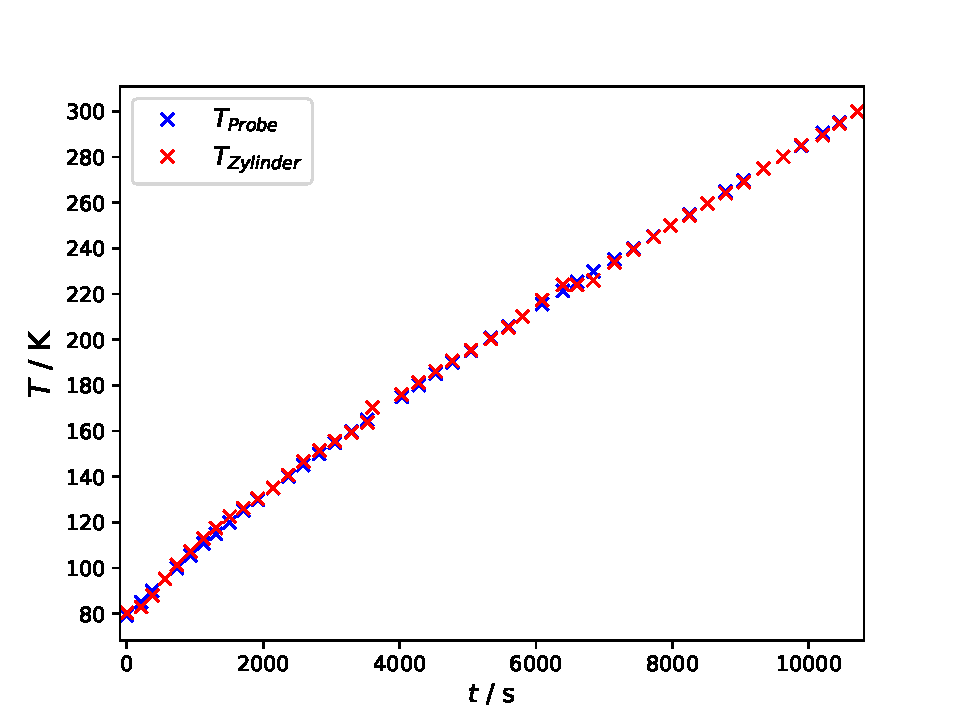
\includegraphics[width = 0.8\textwidth]{Plots/temp.pdf}
  \caption{Temperaturverläufe des Zylinders und der Probe gegenüber der Zeit.
  Häufig Überlappen die Probentemperatur $T_{Probe}$ und die Zylindertemperatur $T_{Zylinder}$,
  sodass nur $T_{Zylinder}$ abgebildet wird.}
  \label{fig:temp}
\end{figure}


\subsection{Wärmekapazität $C\ua{V}$}
\label{sec:wärmekapazität}

Aus der Wärmekapazität bei konstantem Druck $C\ua{p}$ kann
durch den Zusammenhang~\eqref{eqn:c_p-c_v} die Wärmekapazität bei
konstantem Volumen $C\ua{V}$ berechnet werden.

Für das Kompressionsmodul $\kappa$ wird der Wert $\kappa = \SI{140}{\giga\pascal}$
angenommen~\cite{kompression}.
Für den Ausdehnungskoeffizienten $\alpha(T)$ sind Werte in Quelle~\cite{anleitung}
gegeben. Diese werden durch eine Ausgeichsrechnung an ein Polynom dritten Grades
angenähert. Der Verlauf der Ausgeichsfunktion mit den Daten aus Quelle~\cite{anleitung}
ist in Abb.~\ref{fig:alpha} dargestellt.
Der Verlauf der aus den Messdaten errechneten Wärmekapazität $C\ua{V}$
für verschiedene Temperaturen $T$ ist in Abb.~\ref{fig:c_v} erkenntlich.
Es wird ersichtlich, dass in Abb.~\ref{fig:c_v} Werte auftauchen, die sehr
stark erwarteten Trend abweichen.
Diese Abweichung wird auf zwei vermutlich fehlerhafte Messdaten in der Zeitmessung zurückgeführt.
Diese sind in Abb.~\ref{fig:c_v} rot makiert.

\begin{figure}[h]
  \centering
  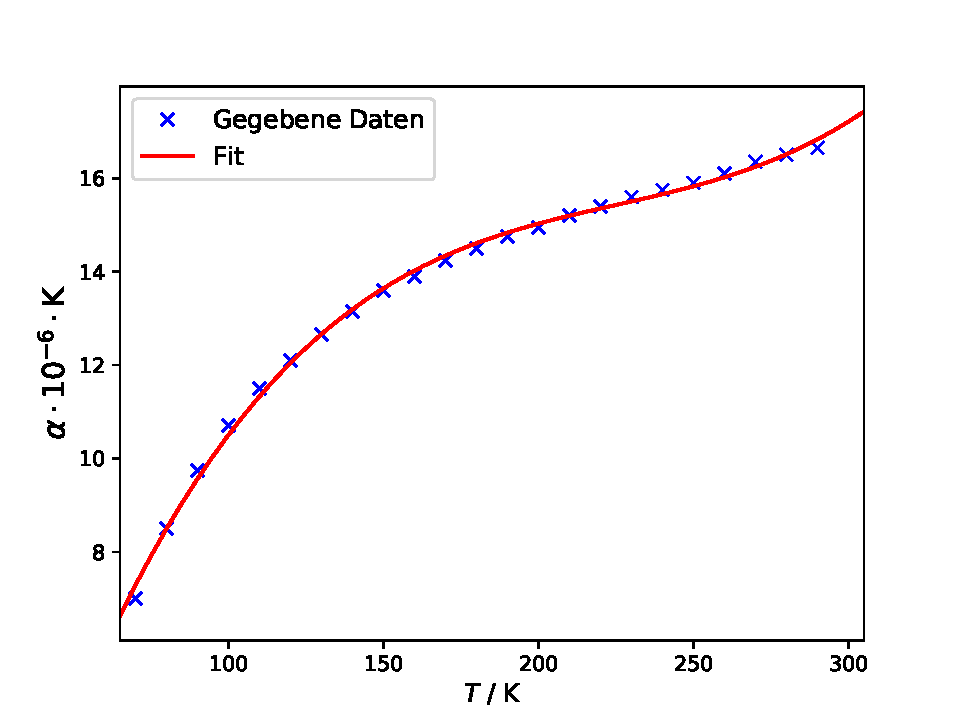
\includegraphics[width = 0.8\textwidth]{Plots/alpha_T.pdf}
  \caption{Ausgeichsfunktion des Ausdehnungskoeffizienten für steigende Temperaturen.}
  \label{fig:alpha}
\end{figure}

\begin{table} 
\centering 
\caption{Messdaten zu der Wärmekapazität $C_p$} 
\label{tab:c_p} 
\begin{tabular}{S@{${}\pm{}$} S S S S S } 
\toprule  
\multicolumn{2}{c}{$C_p / \si{\joule \per \kelvin \per \mol}$} & {$U / \si{\volt}$} & {$ I / \si{\milli\ampere}$} & {$ \increment t / \si{\s}$} & {$ \increment T / \si{\kelvin}$}  \\ 
\midrule  
15.69  & 0.01  & 15.74  & 150.5  & 210  & 5.89\\ 
14.63  & 0.01  & 15.84  & 151.3  & 163  & 4.96\\ 
16.10  & 0.01  & 15.90  & 151.8  & 187  & 5.21\\ 
16.12  & 0.01  & 15.80  & 150.7  & 173  & 4.75\\ 
16.33  & 0.01  & 15.81  & 150.6  & 202  & 5.47\\ 
16.24  & 0.01  & 15.84  & 150.8  & 192  & 5.25\\ 
18.52  & 0.02  & 15.87  & 151.0  & 179  & 4.30\\ 
17.91  & 0.02  & 15.88  & 151.2  & 202  & 5.03\\ 
17.92  & 0.02  & 15.91  & 151.3  & 202  & 5.04\\ 
19.37  & 0.02  & 15.86  & 150.7  & 210  & 4.81\\ 
19.76  & 0.02  & 15.88  & 150.8  & 225  & 5.07\\ 
19.75  & 0.02  & 15.90  & 150.9  & 225  & 5.08\\ 
19.29  & 0.02  & 15.91  & 151.0  & 220  & 5.09\\ 
21.33  & 0.02  & 15.92  & 151.0  & 232  & 4.86\\ 
20.94  & 0.02  & 15.93  & 151.1  & 228  & 4.87\\ 
21.08  & 0.02  & 15.85  & 150.3  & 244  & 5.12\\ 
21.22  & 0.02  & 15.87  & 150.4  & 234  & 4.89\\ 
6.18  & 0.01  & 15.88  & 150.5  & 75  & 5.39\\ 
40.62  & 0.04  & 15.88  & 150.5  & 427  & 4.67\\ 
21.57  & 0.02  & 15.89  & 150.5  & 251  & 5.17\\ 
22.27  & 0.02  & 15.90  & 150.6  & 247  & 4.94\\ 
22.23  & 0.02  & 15.91  & 150.6  & 247  & 4.95\\ 
23.28  & 0.02  & 15.91  & 150.7  & 272  & 5.20\\ 
22.84  & 0.02  & 15.91  & 150.7  & 293  & 5.71\\ 
23.45  & 0.02  & 15.92  & 150.7  & 262  & 4.98\\ 
21.34  & 0.02  & 15.92  & 150.7  & 203  & 4.24\\ 
23.26  & 0.02  & 15.92  & 150.7  & 287  & 5.50\\ 
23.45  & 0.02  & 15.92  & 150.8  & 303  & 5.76\\ 
22.98  & 0.02  & 15.92  & 150.8  & 207  & 4.02\\ 
23.75  & 0.02  & 15.93  & 150.8  & 241  & 4.53\\ 
27.25  & 0.02  & 15.92  & 150.8  & 308  & 5.04\\ 
24.28  & 0.02  & 15.92  & 150.8  & 275  & 5.05\\ 
25.18  & 0.02  & 15.92  & 150.9  & 300  & 5.32\\ 
24.24  & 0.02  & 15.92  & 150.9  & 248  & 4.57\\ 
24.32  & 0.02  & 15.92  & 150.9  & 277  & 5.08\\ 
24.35  & 0.02  & 15.92  & 150.9  & 264  & 4.84\\ 
23.43  & 0.02  & 15.92  & 150.9  & 268  & 5.11\\ 
24.34  & 0.02  & 15.92  & 150.9  & 265  & 4.86\\ 
25.43  & 0.02  & 15.92  & 150.9  & 292  & 5.13\\ 
25.10  & 0.02  & 15.91  & 150.9  & 289  & 5.14\\ 
23.82  & 0.02  & 15.91  & 151.0  & 261  & 4.89\\ 
24.78  & 0.02  & 15.91  & 151.0  & 315  & 5.67\\ 
24.79  & 0.02  & 15.91  & 151.0  & 244  & 4.39\\ 
23.68  & 0.02  & 15.91  & 151.0  & 261  & 4.92\\ 
\bottomrule 
\end{tabular} 
\end{table}

\FloatBarrier
\begin{figure}
  \centering
  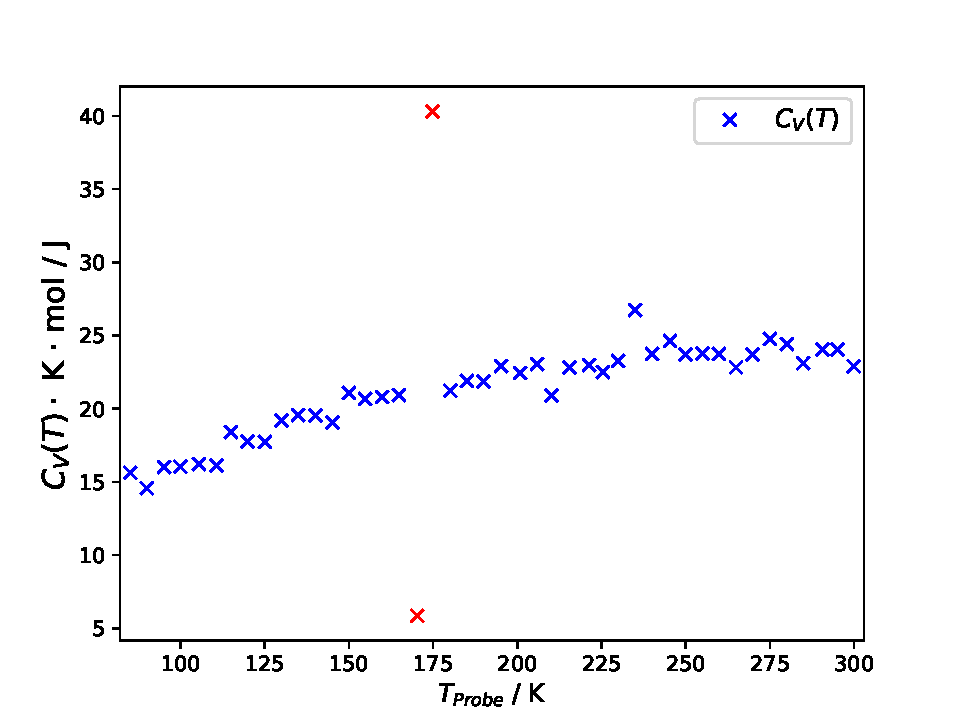
\includegraphics[width = 0.8\textwidth]{Plots/C_V_korrektur.pdf}
  \caption{Daten der Wärmekapazität für steigende Temperaturen. Rot eingefärbte Punkte symbolisieren die vermuteten fehlerhaften Messdaten.}
  \label{fig:c_v}
\end{figure}

\subsection{Debye-Funktion}

In Quelle~\cite{anleitung} sind die Werte der Funktion $C\ua{V} = f\left(\frac{\theta\ua{D}}{T}\right)$
angegeben. Die ermittelten Wärmekapazitäten $C\ua{V}(T)$ können
mit den Daten der Wertetabelle verglichen werden, sodass
der zugehörige $\left(\frac{\theta\ua{D}}{T}\right)$--Wert nach Multiplikation
mit der Temperatur $T$ die Debye-Temperatur ergibt.
Die gefundenen Debye-Temperaturen sind in Tab.~\ref{tab:debye} angegeben.
Es wird angenommen, dass das Verhältnis von $\frac{\theta_{\symup{D}}}{T}$
bis auf $\pm 0,1$ bekannt ist.
Dabei werden nur Wärmekapazitäten bis zu $T = \SI{170}{\kelvin}$ berücksichtigt.\\
Der experimentelle Wert der Debye-Temperatur $\theta\ua{D, exp}$ ergibt sich aus dem gewichteten Mittelwert
der Debye-Temperaturen aus Tabelle~\ref{tab:debye}.

\begin{equation}
  \label{eqn:debye}
  \theta\ua{D, exp} \approx \SI{311.7(125)}{\kelvin}
\end{equation}

\subsection{Berechnung von $\omega\ua{D}$ und $\theta\ua{D}$}

Die Debye-Frequenz $\omega\ua{D}$ wird wie in dem Abschnitt~\ref{sec:debye} beschrieben mit Formel~\eqref{eqn:omega_D}
errechnet.
Für die einzelnen Größen ergeben sich die folgenden Werte.

\begin{align*}
  m\ua{Probe} &= \SI{342}{\gram} \text{~\cite{anleitung}}\\
  M\ua{Cu} &= \num{63.55}\su{u}\cdot N\ua{A} \text{~\cite{cu_mass}}\\
  v\ua{l} &= \SI{4.7}{\meter\per\second}\\
  v\ua{t} &= \SI{2.26}{\meter\per\second}\\
  N_L &= \num{3.24e24} \\
  V &= L^3 = V_0\cdot\frac{m}{M}\approx \SI{0.382}{\centi\meter^3}\\
  \omega\ua{D} &\approx \SI{43.5e12}{\per\second}\\
  \theta\ua{D} &\approx \SI{322.21}{\kelvin}
\end{align*}

\section{Diskussion}
\label{sec:diskussion}

In diesem Kapitel werden die Messergebnisse diskutiert und Abweichungen zu den Theoriewerten untersucht.
Der Mittelwert der experimentell gefundenen Debye-Temperaturen $\theta\ua{D, exp}$ ist ca.
$\num{5.9}\,\%$ kleiner als der Theoriewert $\theta\ua{D}$, doch liegt im Rahmen der
Standardabweichung.
Allgemein könnten Abweichung durch eine ungleiche Wärmeabstrahlung von Probe und Zylinder
erklärt werden, welche darauf beruhen könnte, dass beispielsweise das Kupfer
des Zylinders eine dickere Oxiedschicht besitzt. Damit wäre die Emissivität ungleich
der Probenemissivität, sodass die abgestrahlte Wärme der Probe ungleich der
zurückgestrahlten Wärme des Zylinders wäre.
Darüberhinaus ist nicht sichergestellt, dass Wärmeverluste durch
Wärmeleitung über die Halterungen der Probe ausgeschlossen sind.
Es fällt auf, dass zwei Messdaten von $C\ua{V}$ den Dulong-Petit-Wert von
$3R \approx \SI{24.942}{\joule\per\kelvin\per\mol}$ überschreiten.
Das asymptotische Verhalten der Wärmekapazität $C\ua{V}$ gegen den
Dulong-Petit-Wert in Abb. \ref{fig:c_v} ist dennoch zu erkennen.

\newpage
\pagestyle{empty}
\section{Tabellen}
\label{sec:tabellen}
\begin{table}[H]
\centering 
\caption{Ergebnisse der Wärmekapazität $C_V$.} 
\label{tab:c_v} 
\begin{tabular}{S@{${}\pm{}$} S S@{${}\pm{}$} S } 
\toprule  
\multicolumn{2}{c}{$C_V / \si{\joule \per \kelvin \per \mol}$} & \multicolumn{2}{c}{$ \alpha / \si{10^6\kelvin}$} \\ 
\midrule  
15.63  & 0.02  & 8.40  & 1.11\\ 
14.56  & 0.02  & 9.05  & 1.19\\ 
16.01  & 0.03  & 9.57  & 1.25\\ 
16.03  & 0.03  & 10.07  & 1.33\\ 
16.22  & 0.03  & 10.50  & 1.40\\ 
16.11  & 0.04  & 10.97  & 1.48\\ 
18.38  & 0.04  & 11.38  & 1.56\\ 
17.76  & 0.05  & 11.70  & 1.63\\ 
17.74  & 0.05  & 12.05  & 1.72\\ 
19.19  & 0.06  & 12.37  & 1.81\\ 
19.56  & 0.06  & 12.66  & 1.90\\ 
19.53  & 0.07  & 12.94  & 1.99\\ 
19.06  & 0.08  & 13.20  & 2.09\\ 
21.08  & 0.09  & 13.44  & 2.20\\ 
20.68  & 0.09  & 13.64  & 2.30\\ 
20.80  & 0.10  & 13.84  & 2.41\\ 
20.92  & 0.11  & 14.02  & 2.52\\ 
5.86  & 0.12  & 14.19  & 2.64\\ 
40.29  & 0.14  & 14.35  & 2.77\\ 
21.23  & 0.14  & 14.48  & 2.88\\ 
21.91  & 0.16  & 14.61  & 3.02\\ 
21.86  & 0.17  & 14.73  & 3.15\\ 
22.89  & 0.18  & 14.84  & 3.28\\ 
22.44  & 0.20  & 14.94  & 3.43\\ 
23.03  & 0.21  & 15.05  & 3.59\\ 
20.90  & 0.22  & 15.13  & 3.74\\ 
22.81  & 0.24  & 15.20  & 3.87\\ 
22.98  & 0.26  & 15.29  & 4.05\\ 
22.50  & 0.27  & 15.38  & 4.23\\ 
23.26  & 0.29  & 15.44  & 4.37\\ 
26.74  & 0.31  & 15.50  & 4.52\\ 
23.75  & 0.33  & 15.58  & 4.70\\ 
24.64  & 0.35  & 15.66  & 4.88\\ 
23.68  & 0.37  & 15.75  & 5.08\\ 
23.74  & 0.40  & 15.83  & 5.26\\ 
23.75  & 0.42  & 15.92  & 5.45\\ 
22.81  & 0.45  & 16.02  & 5.65\\ 
23.70  & 0.48  & 16.13  & 5.86\\ 
24.77  & 0.51  & 16.24  & 6.06\\ 
24.41  & 0.54  & 16.37  & 6.28\\ 
23.12  & 0.57  & 16.52  & 6.51\\ 
24.04  & 0.61  & 16.67  & 6.73\\ 
24.02  & 0.65  & 16.86  & 6.99\\ 
22.89  & 0.69  & 17.02  & 7.20\\ 
\bottomrule 
\end{tabular} 
\end{table}
\begin{table}[H]
\centering 
\caption{Gefundene Werte von $\theta_{\symup{D}}$.} 
\label{tab:debye} 
\begin{tabular}{S@{${}\pm{}$} S S@{${}\pm{}$} S S S } 
\toprule  
\multicolumn{2}{c}{$\theta_{\symup{D}} / \si{\kelvin}$} & \multicolumn{2}{c}{$C_V / \si{\joule \per \kelvin \per \mol}$} & {$T / \si{\kelvin}$} & {$\frac{\theta_{\symup{D}}}{T}$}  \\ 
\midrule 
272.20  & 8.51  & 15.63  & 0.02  & 85.06  & 3.20\\ 
315.08  & 9.00  & 14.56  & 0.02  & 90.02  & 3.50\\ 
295.22  & 9.52  & 16.01  & 0.03  & 95.23  & 3.10\\ 
309.93  & 10.00  & 16.03  & 0.03  & 99.98  & 3.10\\ 
326.90  & 10.55  & 16.22  & 0.03  & 105.45  & 3.10\\ 
343.16  & 11.07  & 16.11  & 0.04  & 110.70  & 3.10\\ 
293.25  & 11.50  & 18.38  & 0.04  & 115.00  & 2.55\\ 
324.09  & 12.00  & 17.76  & 0.05  & 120.03  & 2.70\\ 
337.70  & 12.51  & 17.74  & 0.05  & 125.08  & 2.70\\ 
305.24  & 12.99  & 19.19  & 0.06  & 129.89  & 2.35\\ 
317.15  & 13.50  & 19.56  & 0.06  & 134.96  & 2.35\\ 
329.08  & 14.00  & 19.53  & 0.07  & 140.03  & 2.35\\ 
333.78  & 14.51  & 19.06  & 0.08  & 145.12  & 2.30\\ 
284.97  & 15.00  & 21.08  & 0.09  & 149.98  & 1.90\\ 
309.70  & 15.49  & 20.68  & 0.09  & 154.85  & 2.00\\ 
303.95  & 16.00  & 20.80  & 0.10  & 159.97  & 1.90\\ 
313.25  & 16.49  & 20.92  & 0.11  & 164.87  & 1.90\\ 
\bottomrule 
\end{tabular} 
\end{table}
